\documentclass[final]{beamer}
% http://tex.stackexchange.com/questions/56205/wrapfigure-beamer-style
\usepackage{color}
%\usepackage{cutwin}
%\usetheme{RJH}
\usetheme{Berkeley}
%\usetheme{Bergen}
\usepackage[orientation=portrait,size=a0,scale=1.4,debug]{beamerposter}
\usepackage[absolute,overlay]{textpos}
\setlength{\TPHorizModule}{1cm}
\setlength{\TPVertModule}{1cm}
\beamertemplatenavigationsymbolsempty
% RGB (145,201,219), #91C9DB
%\definecolor{mybluelabel}{RGB}{145,201,219}
% RGB (48,174,228), #30AEE4
\definecolor{mybluelabel}{RGB}{48,174,228}

%\title{Data-Intensive Analysis for High Energy Physics (DIANA/HEP)}
%\author{Peter Elmer}
%\date{}

\begin{document}
\begin{frame}{} 

\begin{textblock}{20}(2,2)
\begin{center}
\begin{figure}[tbph]
\centering
%
\includegraphics[width=0.45\textwidth]{images/dianahep-logo.png}

\includegraphics[width=0.70\textwidth]{images/diana-hep-06-logo-horizontal.png}
\end{figure}
\href{http://diana-hep.org}{http://diana-hep.org}
%\url{http://diana-hep.org}
\end{center}
\end{textblock}


\begin{textblock}{84.0}(6,2)
\begin{center}
\begin{LARGE}
Data-Intensive Analysis for High Energy Physics (DIANA/HEP)
\end{LARGE}
\end{center}
\end{textblock}

\begin{textblock}{84.0}(6,5)
\begin{center}
\begin{Large}
PIs: Peter Elmer (Princeton U.), Brian Bockelman (U.Nebraska-Lincoln), \\ 
Kyle Cranmer (NYU), Mike Sokoloff (U.Cincinnati)
\end{Large}
\end{center}
\end{textblock}

\begin{textblock}{38.0}(4,10)
\begin{block}{High Energy Physics (HEP)}
%\begin{center}
The quest to understand the fundamental building blocks of nature,
and their interactions, is one of the longest running and most
ambitious of human endeavors. Facilities such as the Large Hadron
Collider (LHC), where we do our research, represent a huge step
forward in our ability to answer these questions. The discovery of
the Higgs boson, the observation of exceedingly rare decays of B
mesons, and exclusion of countless theories beyond the Standard
Model (SM) of particle physics demonstrate that these experiments
deliver results. However, the most interesting fundamental physics
questions remain wide open, amongst them: What is the dark matter
which pervades the universe? Does space-time have additional
symmetries or extend beyond the 3 spatial dimensions we know? What
is the mechanism stabilizing the Higgs mass from enormous quantum
corrections? Are neutrinos, whose only SM interactions are weak,
their own anti-particles? Can the theories of gravity and quantum
mechanics be reconciled?
%questions remain wide open, amongst them: 
%\begin{itemize} 
%\item What is the dark matter which pervades the universe? 
%\item Does space-time have additional symmetries or extend beyond the 3 spatial dimensions we know? 
%\item What is the mechanism stabilizing the Higgs mass from enormous quantum
%corrections? 
%\item Are neutrinos, whose only SM interactions are weak, their own anti-particles? 
%\item Can the theories of gravity and quantum mechanics be reconciled?
%\end{itemize} 
~~~ \\
\begin{figure}[tbph]
\centering
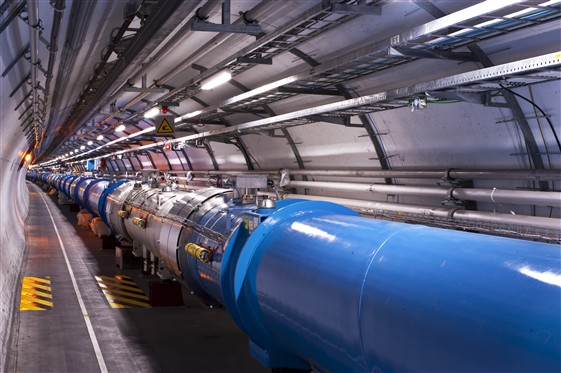
\includegraphics[width=0.48\textwidth]{images/0910152_02-A5-at-72-dpi.jpg}
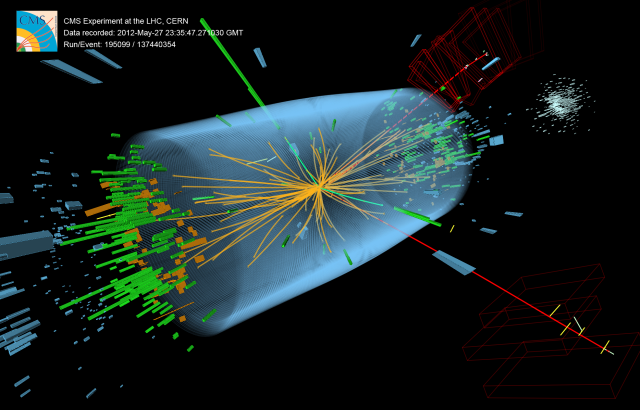
\includegraphics[width=0.50\textwidth]{images/eemm_run195099_evt137440354_ispy_3d-annotated-2.png}
\begin{center}
{\footnotesize \copyright~2009-2016 CERN (License: CC-BY-SA-4.0)}
\end{center}
\end{figure}
\end{block}
\end{textblock}

%\begin{textblock}{38.0}(4,10)
\begin{textblock}{38.0}(44,10)
\begin{block}{The DIANA/HEP Project}
The primary goal of DIANA/HEP is to develop state-of-the-art tools
for experiments which acquire, reduce, and analyze petabytes of
data. Improving performance, interoperability, and collaborative
tools through modifications and additions to ROOT and other packages
broadly used by the community will allow users to more fully exploit
the data being acquired at CERN's LHC and
other facilities. The LHC experiments, for example, use nearly 0.5 Exabyte of
storage today, and planned upgrades through the 2020s will increase this
by more than a factor of 100. 
\end{block}
\end{textblock}

\begin{textblock}{38.0}(44,25.5)
\begin{block}{The HEP Analysis Software Ecosystem}
ROOT (\href{https://root.cern.ch}{https://root.cern.ch}) is
home for most community analysis
software developed in particle physics and related fields. Begun at CERN in 1995,
it provides a sophisticated data format and serialization technology
as well as key software tools for
data modeling, likelihood fitting, statistics and
multivariate data analysis. It also has a broader range of
functionalities, not strictly tied to the data-intensive aspects,
including interactive C++ analysis, histogramming,
graphics, math libraries, image manipulation,
and tools for distributed computing. 
%Despite many
%innovative features, the components are seen as too coupled,
%and limited by design decisions taken 20 years ago.
Given the challenges from technology evolution and analysis complexity,
%large changes are needed,
%much as ROOT replaced an earlier generation of
%FORTRAN-based tools.
DIANA/HEP is building on and improving these
community libraries, moving other existing software elements into
community libraries, and developing additional new tools. We are also working to strengthen and grow the wider HEP software development community by building sustainable collaborations which extend beyond the DIANA/HEP project.
\end{block}
\end{textblock}





\begin{textblock}{78.0}(4,49)
\begin{block}{Project Status}
\end{block}
\end{textblock}

\begin{textblock}{22.5}(5.5,52.5)
\textcolor{mybluelabel}{\bf Improved Performance} \\
To reduce the time to scientific discovery and to enable more in-depth analyses, we are increasing the rate of access to ROOT data files. This includes streamlined access to simpler data types (uproot and BulkIO) and faster compression algorithms (LZ4 and ZSTD). These efforts have already provided factors-of-several improvements.
\end{textblock}

\begin{textblock}{12.5}(29,53)
\begin{figure}[tbph]
\centering
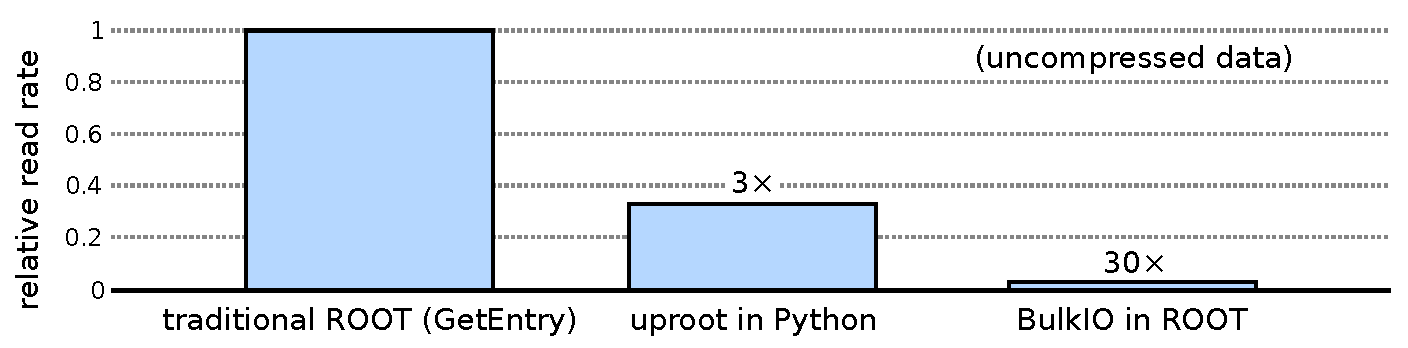
\includegraphics[width=\textwidth]{images/getentry-uproot-bulkio.pdf}

\vspace{0.5 cm}
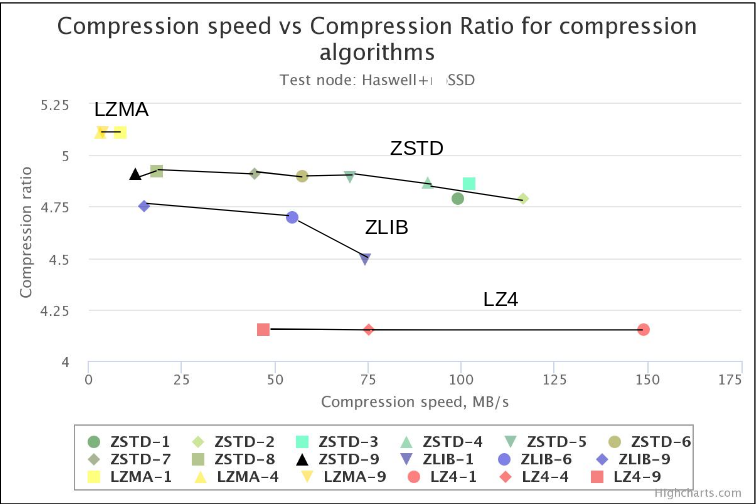
\includegraphics[width=\textwidth]{images/compr.png}
\end{figure}
\end{textblock}

%%%

\begin{textblock}{22.5}(5.5,67.5)
\textcolor{mybluelabel}{\bf Bridging to Big Data} \\
``Big Data'' software in industry, such as the Spark and scientific Python ecosystems, both complement and reproduce functionality of software traditionally developed within HEP. To give physicists more options and reduce maintenance burdens within HEP, DIANA is building bridges between HEP software and the Big Data ecosystems: \href{https://github.com/diana-hep/spark-root}{Spark-ROOT} to Spark and \href{https://github.com/scikit-hep/uproot}{uproot}/\href{https://github.com/diana-hep/oamap}{OAMap} to Numpy, Numba, and Dask.
\end{textblock}

\begin{textblock}{12.5}(29,68.5)
\begin{figure}[tbph]
\centering
%
\includegraphics[width=0.8\textwidth]{images/interoperable.jpg}
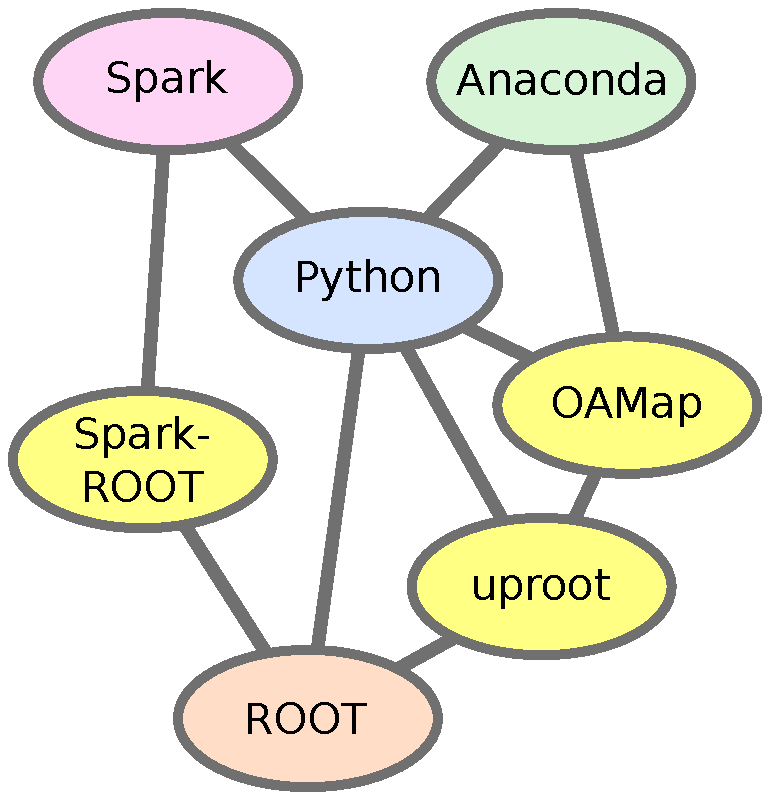
\includegraphics[width=\textwidth]{images/new_relationship.pdf}
\end{figure}
\end{textblock}

%%%

\begin{textblock}{23}(45.5,68)
\textcolor{mybluelabel}{\bf High-Level Tools} \\
Computing issues can get in the way of a focus on physics, especially for new students who must learn both at the same time. We are therefore striving to present HEP analysis with higher-level interfaces. \href{http://scikit-hep.org/}{Scikit-HEP} incorporates HEP techniques in Pythonic idioms, \href{https://github.com/scikit-hep/uproot}{uproot} provides access to ROOT data as Numpy and Pandas abstractions, and \href{https://github.com/diana-hep/oamap}{OAMap} compiles object-centric user code into fast array operations.
\end{textblock}

\begin{textblock}{12.0}(69.5,67)
\begin{figure}[tbph]
\centering

\includegraphics[width=0.8\textwidth]{images/scikit-hep-logo_800.png}

\vspace{1 cm}

\includegraphics[width=0.8\textwidth]{images/uproot-logo.pdf}
\end{figure}
\end{textblock}

\begin{textblock}{22.5}(45.5,52.5)
\textcolor{mybluelabel}{\bf New Statistical Techniques} \\
We are developing of new tools and methods for
high-level statistical analysis in particle physics. Our activities
include research and tools for simulator-based inference (\href{http://diana-hep.org/carl/}{Carl}), machine 
learning for particle physics (\href{https://scikit-optimize.github.io/}{Scikit-Optimize}), high-level software for efficient numerical
computations, and education efforts in these respective domains.
\end{textblock}

\begin{textblock}{12.5}(69,54)
\begin{figure}[tbph]
\centering
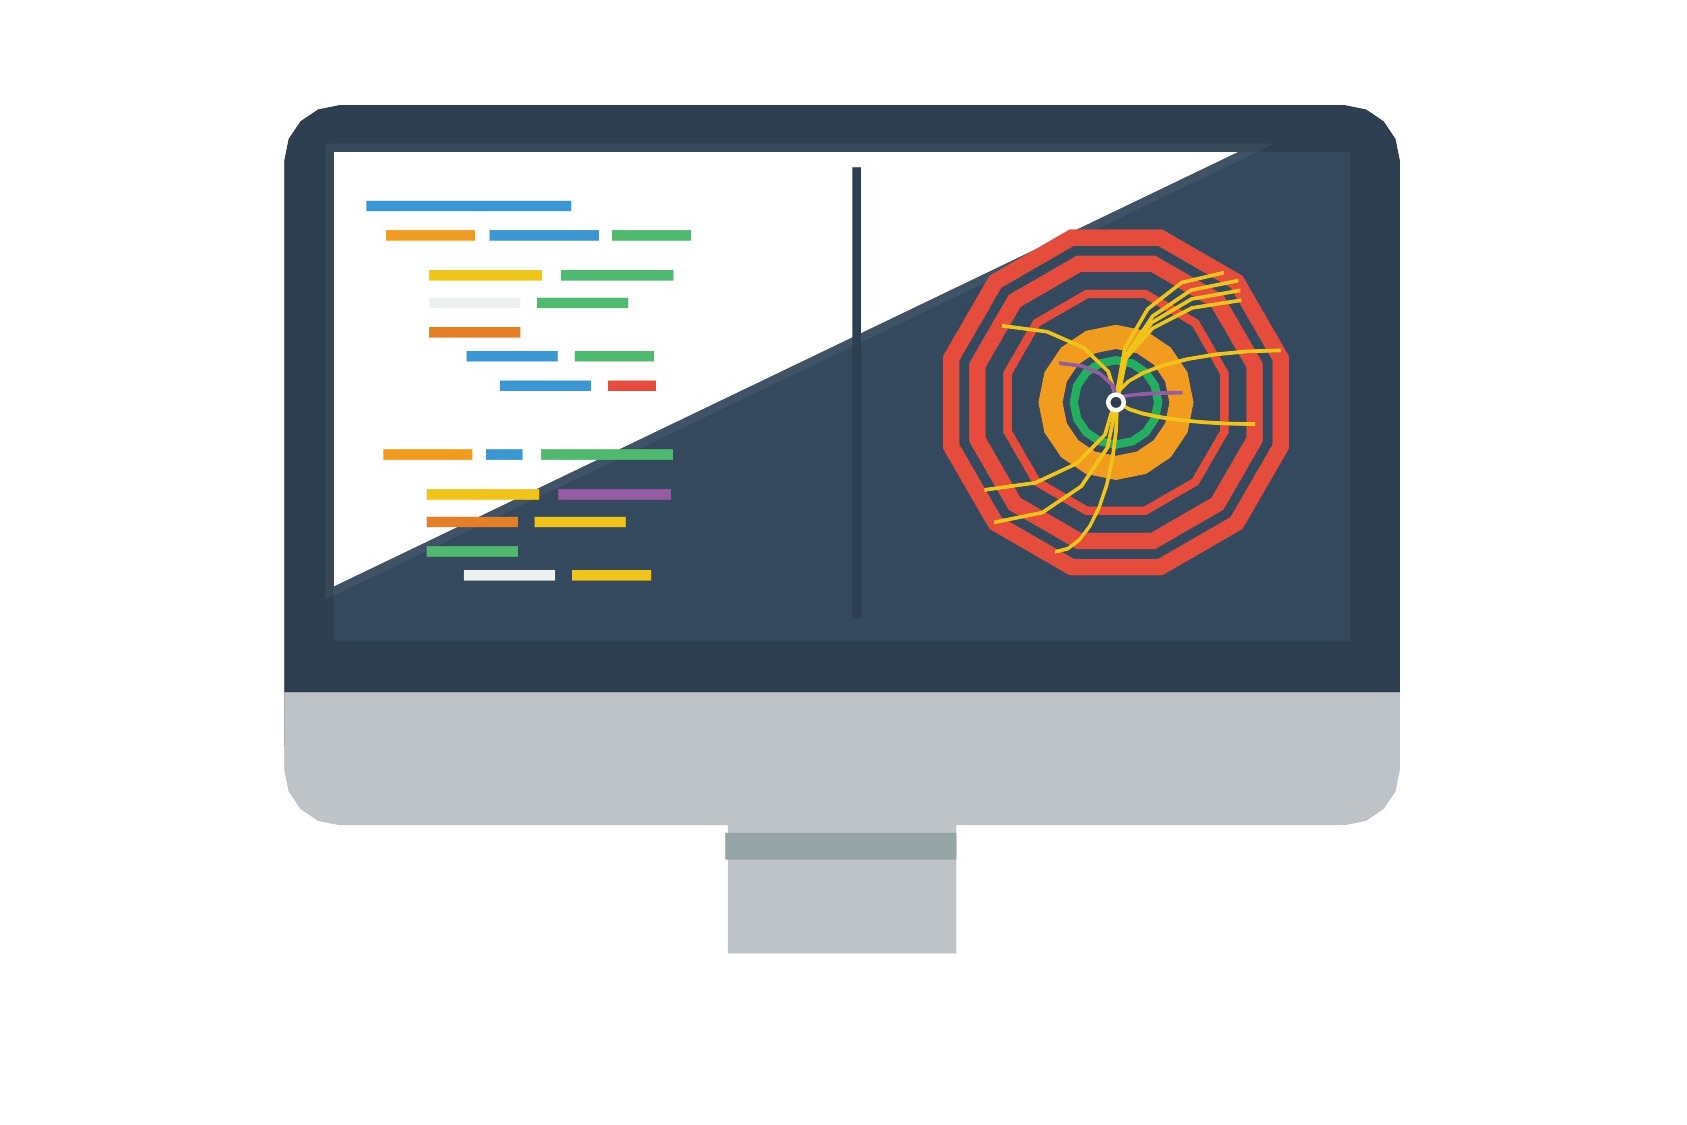
\includegraphics[width=0.9\textwidth]{images/better-software.jpg}
\end{figure}
\end{textblock}

%\begin{textblock}{22.5}(45.5,77)
%\textcolor{mybluelabel}{\bf Training} \\
%Provide training for students in all of our core research topics.
%\end{textblock}

%\begin{textblock}{12.5}(69,77)
%\begin{figure}[tbph]
%\centering
%
\includegraphics[width=0.8\textwidth]{images/training.jpg}
%\end{figure}
%\end{textblock}






\begin{textblock}{38.0}(4,85)
\begin{block}{Project Team}
\begin{itemize}
\item Peter Elmer (Lead PI) - {\it Princeton Univ., Dept. of Physics}
\item Brian P. Bockelman (PI) - {\it Univ. of Nebraska-Lincoln, Dept. of Computer Science and Engineering}
\item Kyle Cranmer (PI) - {\it New York Univ., Dept. of Physics \& Center for Data Science}
\item Michael D. Sokoloff (PI) - {\it Univ. of Cincinnati, Dept. of Physics}
\item Jinyang Li (Senior Personnel) - {\it New York Univ., Computer Science Dept.}
\item David Abdurachmanov - {\it Univ. of Nebraska-Lincoln, Dept. of Computer Science and Engineering}
\item David Lange - {\it Princeton Univ., Dept. of Physics}
\item Gilles Louppe - {\it New York Univ., Dept. of Physics \& Center for Data Science}
\item James Pivarski - {\it Princeton Univ., Dept. of Physics}
\item Eduardo Rodrigues - {\it Univ. of Cincinnati, Dept. of Physics}
\item Zhe Zhang - {\it Univ. of Nebraska-Lincoln, Dept. of Computer Science and Engineering} (Ph.D.\ Student)
\item Chien-Chin Huang - {\it New York Univ., Computer Science Dept.} (Ph.D.\ Student) 
\end{itemize}
\end{block}
\end{textblock}

\begin{textblock}{38.0}(44,85)
\begin{block}{Advisory Board}
\begin{itemize}
\item Amber Boehnlein - {\it CIO, Thomas Jefferson National Accelerator Facility}
\item Katherine Copic - {\it Director of Growth, Insight Data Science}
\item Jacob VanderPlas - {\it Director of Research, Physical Sciences, eScience Institute, Univ. of Washington}
\item Fernando Perez - {\it Staff Scientist, Data Science and Technology Division, Lawrence Berkeley National Laboratory; Associate Researcher, Berkeley Institute for Data Science, UC Berkeley.}
\item Attanagoda Santha - {\it Architect, Fannie Mae}
\end{itemize}
\end{block}
\end{textblock}



\begin{textblock}{38.0}(44,101.5)
\begin{block}{Acknowledgement}
This project is supported by National Science Foundation grants ACI-1450310, ACI-1450319, ACI-1450323, and ACI-1450377. Any opinions, findings, conclusions or recommendations expressed in this material are those of the developers and do not necessarily reflect the views of the National Science Foundation.
\end{block}
\end{textblock}

% http://diana-hep.org/downloads/diana-si2-pi-workshop-2017.pdf
% goo.gl/KxSovq


\begin{textblock}{10.0}(44,112)

\includegraphics[width=0.4\textwidth]{images/si2-2017-poster-qr.png}
\end{textblock}

%\begin{textblock}{18.0}(54,112)
\begin{textblock}{24.0}(50,112)
%
\includegraphics[width=0.45\textwidth]{images/si2-2017-poster-qr.png}
\begin{flushleft}
Online version of this poster with clickable \\
links: \href{http://goo.gl/KxSovq}{http://goo.gl/KxSovq}
\end{flushleft}
\end{textblock}

\begin{textblock}{10.0}(72,111.5)
\begin{flushright}

\includegraphics[width=0.4\textwidth]{images/nsf1.jpg}
\end{flushright}
\end{textblock}


\end{frame}
\end{document}
